% ----------------------------------------------------------
\chapter{DICIONÁRIO DE PROJETO}\label{cap:desenvolvimento}
% ----------------------------------------------------------
Deve-se inserir texto entre as seções.
% ----------------------------------------------------------
\subsection{Lista de Abreviaturas nos Artefatos do Documento}
Lista de Abreviaturas nos Artefatos do Documento
% ----------------------------------------------------------
\begin{quadro}[htb]
	\centering
	\caption{\label{Formatação do texto.}Requisitos funcionais}	
	\begin{tabular}{|p{4cm}|m{3cm}|p{7cm}|}
		\hline
		\textbf{Artefato} & \textbf{Termo ou sigla} & \textbf{Significado} \\ \hline
		Lista de Requisitos & RF & Requisito funcional: Funcionalidades que um sistema deve possuir. \\ \hline
		Lista de Requisitos & RNF & Requisito não funcional: Características que o software deve possuir, não apresenta funcionalidades. \\ \hline
		Lista de Regras de Negócio & RN & Regra de Negócio: Conjunto de diretizes que orientam como deve ser o funionamente das funcionalidades. \\ \hline
	\end{tabular}
	\fonte{\textcite{Elaborado pelos autores(2023)}.}
\end{quadro}


% ----------------------------------------------------------
\chapter{Referencial teórioco}\label{cap:desenvolvimento}
% ----------------------------------------------------------

% ----------------------------------------------------------
\subsection{React Native}
A utilização do framework React Native se dá ao seu crescente crescimento no mercado. Desenvolvido e mantido pela META empresa, que também é dona do Facebook,
a marca por trás do framework traz consigo uma grande confiabilidade. Além disso, a presença de uma grande comunidade por trás do framework disponibiliza vários conteúdos gratuitos pela internet.
A grande tendência para os novos aplicativos móveis é que sejam desenvolvidos principalmente para as plataformas Android e IOS. Com a utilização do React Native, 
é possível realizar o desenvolvimento híbrido. Conforme (\textcite{Sabino}), "aplicações híbridas são aplicações multiplataforma que permitem a construção 
simultânea de um produto para iOS e Android, em vez de desenvolver duas vezes usando a linguagem nativa de cada plataforma".

Outro fator determinante na escolha da utilização do framework é a sua curva de aprendizado. Por utilizar a linguagem Javascript, a sua familiaridade e popularidade 
no mundo do desenvolvimento é bastante evidente (Figura 1), o que mostra a sua força e importância no mercado.

\begin{figure}[htb]
	\caption{\label{fig:Fig_1}Linguagem de programção}
	\begin{center}
		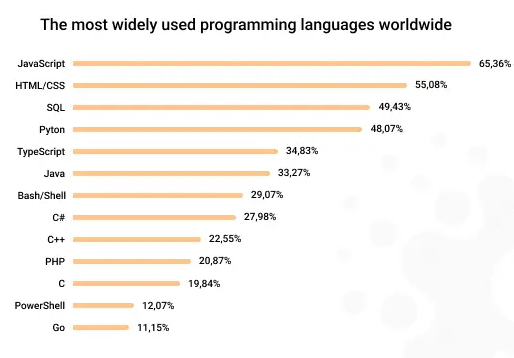
\includegraphics{images/top.png}
	\end{center}
	\fonte{stackoverflow}
\end{figure}
% ----------------------------------------------------------
